% Kompilasi dengan XeLaTeX: latexmk -xelatex 2026-10-20.tex
\documentclass[10.5pt,a4paper]{article}

\usepackage[indonesian]{babel}
\usepackage{fontspec}
\IfFontExistsTF{Calibri}{\setmainfont{Calibri}}{\setmainfont{Carlito}}
\setmonofont{DejaVu Sans Mono}[Scale=0.82]
\usepackage[margin=2cm]{geometry}
\usepackage{microtype}
\usepackage{xcolor}
\usepackage{graphicx}
\usepackage{tikz}
\usetikzlibrary{positioning,fit,backgrounds,arrows.meta,calc}
\usepackage{pgfplots}
\pgfplotsset{compat=1.18}
\usepgfplotslibrary{dateplot,fillbetween}
\usepackage{booktabs,tabularx,array,multirow,longtable}
\usepackage{enumitem}
\usepackage[most]{tcolorbox}
\usepackage{fancyvrb}
\usepackage[hidelinks]{hyperref}
\usepackage{titlesec}

% Gaya bersama diagram (dipakai laporan progress dan deck). Warna anggota sama dengan jobdesc.tex.
\providecolor{izma}{RGB}{31,94,170}
\providecolor{genis}{RGB}{40,130,70}
\providecolor{alif}{RGB}{190,90,20}
\providecolor{shania}{RGB}{140,60,150}
\providecolor{lama}{RGB}{110,110,110}
\providecolor{merah}{RGB}{185,40,40}
\tikzset{
  kotak/.style={draw, rounded corners=3pt, align=center, font=\footnotesize, inner sep=4pt, line width=0.8pt, minimum height=0.9cm},
  milik/.style={kotak, draw=#1, fill=#1!10},
  abu/.style={kotak, draw=lama, fill=black!4},
  panah/.style={-{Stealth[length=2mm]}, line width=0.7pt, draw=black!70},
  putus/.style={panah, dashed},
  label/.style={font=\scriptsize\itshape, text=black!70, fill=white, inner sep=1pt},
  wadah/.style={draw=#1!60, fill=#1!4, rounded corners=5pt, line width=0.6pt, inner sep=6pt},
}

\newcommand{\diagram}[1]{\input{../presentasi/diagram/#1.tex}}
\newcommand{\datafile}[1]{../presentasi/data/#1}
\newcommand{\tbd}[1]{\textcolor{merah}{[TBD: #1]}}
\newcommand{\cmd}[1]{\texttt{#1}}

\titleformat{\section}{\large\bfseries\color{izma}}{\thesection.}{0.5em}{}
\titleformat{\subsection}{\normalsize\bfseries}{\thesubsection}{0.5em}{}
\setlist{nosep, leftmargin=1.4em}
\setlength{\parindent}{0pt}
\setlength{\parskip}{4pt}

\newtcolorbox{ringkas}[1][]{colback=izma!5, colframe=izma, boxrule=0.8pt, arc=3pt, left=6pt, right=6pt, top=4pt, bottom=4pt, fonttitle=\bfseries, title={#1}}
\newtcolorbox{perhatian}[1][]{colback=merah!5, colframe=merah!80!black, boxrule=0.8pt, arc=3pt, left=6pt, right=6pt, top=4pt, bottom=4pt, fonttitle=\bfseries, title={#1}}
\newtcolorbox{langkah}[1][]{colback=genis!5, colframe=genis, boxrule=0.8pt, arc=3pt, left=6pt, right=6pt, top=4pt, bottom=4pt, fonttitle=\bfseries, title={#1}}
\DefineVerbatimEnvironment{terminal}{Verbatim}{fontsize=\footnotesize, frame=single, framesep=4pt, rulecolor=\color{black!30}}

\begin{document}
\sloppy\setlength{\emergencystretch}{3em}

% ======================================================================
\begin{center}
{\LARGE\bfseries Laporan Progress dan User Guide}\\[3pt]
{\large Jalur AI dan Integrasi --- Wind Edge Chip (Tim Chitato)}\\[2pt]
{\normalsize DeepTech for Smart-X Hackathon 2026 \textbullet{} 20 Oktober 2026, diperbarui Rabu 21 Oktober sore (v3) \textbullet{} Izma Alhazmi Herdian}
\end{center}

\vspace{4pt}
\begin{ringkas}[Ringkasan hari ini]
\begin{itemize}
  \item \textbf{Data siap pakai.} 9 file database turbin (13 Jan--20 Okt) dirapikan jadi CSV seragam, lalu dibersihkan menjadi
        \textbf{181.228 menit} data (30 Mar--20 Okt). Ditemukan dan ditangani: sel rusak akibat Excel, anemometer Arduino macet,
        dan \textbf{2.787 reboot Raspi karena internet mati} (penyebab utama celah data).
  \item \textbf{Fitur 2, prediksi daya 1 jam (inti proposal):} MLP 16-32-16-1 \textbf{INT8} dilatih langsung dengan aritmetika RTL FPGA.
        Data uji 1--20 Okt: \textbf{RMSE 10,25 W}, \textbf{skill +0,40} terhadap persistence; lebih baik dari semua baseline
        dan dari versi float-nya sendiri. Bobot ini \textbf{lulus regresi Verilog} (iverilog, 2.000 vektor acak + 597 vektor nyata, 0 beda), bitstream Tang Nano 4K sudah dibangun (LUT 24\%, Fmax 85,7 MHz) dan \textbf{di-flash ke papan} (CRC sukses).
  \item \textbf{Fitur 1, status turbin (SVM TA):} direproduksi (97,6\%, klaim TA 98,22\%), lalu diperbaiki dan
        ditambah deteksi berbasis kurva daya.
  \item \textbf{Fitur 3, setelah inverter/baterai (masukan PLN):} daftar data yang harus diukur, plus simulasi rantai
        angin $\to$ DC $\to$ baterai $\to$ AC.
  \item \textbf{Akses sistem:} Raspi turbin dan Node-RED server bisa dibuka dari laptop (SSH/VS Code). Programnya sudah
        disalin ke repo. Bagian II berisi panduan langkah demi langkah.
\end{itemize}
\end{ringkas}

\begin{ringkas}[Pembaruan 21 Okt siang--sore (v3)]
\begin{itemize}
  \item \textbf{Chip jalan di papan dan live:} HIL ESP32-S3 $\leftrightarrow$ Tang Nano 4K 5.373/5.373 identik; sejak 11.56 chip menghitung prediksi live (\S\ref{sec:fpga}). Bitstream 21 Okt ditulis ke flash FPGA.
  \item \textbf{Model offline} (tanpa Open-Meteo): MAE 5,62 W vs 5,48 W; dipakai otomatis di Node-RED dan ESP32 bila prakiraan kosong (\S\ref{sec:v3}).
  \item \textbf{Pengukur daya komputasi:} ESP32 klasik + 2$\times$ INA219 (Raspi, FPGA + ESP32-S3) $\to$ MQTT \cmd{WEC/daya} $\to$ panel dashboard; tersambung lewat eduroam, menunggu kabel catu dilewatkan INA (\cmd{docs/demo/pemasangan-ina219.png}).
  \item \textbf{Eksperimen M per lapisan:} tidak menurunkan galat, bukan prioritas RTL (\S\ref{sec:v3}).
  \item \textbf{Bahan Demo Day:} rubrik demo (80\% nilai akhir) dipetakan ke deck; \cmd{pitch.pdf} 11 slide + naskah, QnA juri, bahan mentoring hari 2.
\end{itemize}
\end{ringkas}

\begin{ringkas}[Pembaruan 21 Okt (v2)]
\begin{itemize}
  \item \textbf{Dashboard \cmd{/dashboard/hackathon}} (menggantikan \cmd{/v2}): gaya cloaked.com, hero dengan prediksi live, pita gelap tiga fitur ML, CCTV berdampingan dengan digital twin 3D. Dashboard Genis tidak diubah (\S\ref{sec:dash}).
  \item \textbf{Mesin ML tidak lagi tertahan ``menunggu''.} Saat PZEM diam, daya diganti daya wajar dari MLP kurva daya: uji 1--20 Okt (11.166 menit yang sama) \textbf{MAE 4,72 W} vs 4,76 W mode normal (persistence 6,88 W). Riwayat 240 menit disimpan ke MQTT \emph{retained} sehingga deploy/restart tidak mengulang pemanasan.
  \item \textbf{Fitur 1 versi INT8:} MLP kurva daya wajar 16-32-16-1 dengan aritmetika RTL yang sama (MAE 2,57 W), lulus RTL tanpa mengubah datapath (\S\ref{sec:f1int8}).
  \item \textbf{Firmware ESP32-S3} (\cmd{edge/esp32/}): sensor RS-485, 16 fitur INT8, UART ke FPGA + cadangan CPU bit-exact, status, baterai + relai, MQTT + antrean offline. Inti C++ 0 beda terhadap Python/JS; build lulus; \textbf{belum diuji di papan} (\S\ref{sec:esp32}).
  \item \textbf{InfluxDB lokal} + dashboard 11 panel; bug nama field PZEM (huruf kecil) di subscriber diperbaiki (\S\ref{sec:influx}).
  \item \textbf{Temuan lapangan 21 Okt:} PZEM tidak merespons sejak 00.13; Raspi reboot karena internet mati pukul 07.00 dan 07.10.
  \item \textbf{Bisnis:} segmen, aliran pendapatan, komponen inti per turbin $\approx$Rp624 rb dari RAB, dan strategi substitusi impor (\S\ref{sec:bisnis}).
  \item \textbf{Chip jalan di papan:} HIL ESP32-S3 $\leftrightarrow$ Tang Nano 4K \textbf{5.373/5.373 inferensi identik}, 309 siklus; sejak 11.56 chip asli menghitung prediksi live dan hasilnya tampil di dashboard (\S\ref{sec:fpga}).
  \item \textbf{Demo terintegrasi:} \cmd{edge/bridge/fpga\_bridge.py} membawa 16 byte fitur live ke Tang Nano 4K (USB-TTL) atau golden model (\cmd{--sim}) dan menampilkan hasil chip di dashboard; runbook di \cmd{docs/demo/runbook.md}; mode demo digital twin diperbaiki (sebelumnya crash karena \cmd{Object.freeze}).
\end{itemize}
\end{ringkas}

\begin{perhatian}[Yang dibutuhkan dari anggota tim]
\begin{tabularx}{\linewidth}{@{}l X@{}}
\textcolor{alif}{\textbf{Alif}}   & (1) Tinjau branch \cmd{feature/integrasi} (RTL + bobot training, regresi Verilog sudah lulus; Makefile Linux
                                    + \cmd{run\_regression\_real.py}). (2) Format UART sudah disepakati lewat RTL 21 Okt (paket 19 B/7 B + CRC-8, 921600 bps); firmware, jembatan, dan \cmd{docs/kontrak-uart.md} sudah mengikuti. (3) M/S per lapisan sudah diuji dan tidak menurunkan galat (lihat \S\ref{sec:fpga}); tidak perlu diubah. (4) Flash Tang Nano 4K sekarang berisi bitstream 21 Okt dengan bobot hasil latih (HIL lulus); sebelum build ulang, jalankan \cmd{run\_regression\_real.py} agar \cmd{hw/rtl/*.hex} berisi bobot latih. (5) Atur \cmd{git config user.name/email} (commit tercatat ``Your Name''). \\
\textcolor{genis}{\textbf{Genis}} & (1) Ekspor ulang CSV langsung dari Google Sheets untuk 26 Apr--1 Okt (data rusak oleh Excel).
                                    (2) Diameter rotor \textbf{ditetapkan 2,5 m} (keputusan tim 21 Okt; TA menulis 3 m). Catatan: dengan angin stasiun dan 2,5 m, $\pm$28\% menit Okt punya Cp $>$ 0,59, sehingga SVM tetap sering ``Anomaly''.
                                    (3) Rakit ESP32-S3 + modul RS-485 (firmware \cmd{edge/esp32/} sudah siap, pin di README). (4) Turbin 2 (\cmd{TurbinAngin2}): turbin mana, sejak kapan?
                                    (5) PZEM tidak merespons sejak 21 Okt 00.13: cek kabel/catu PZEM. \\
\textcolor{shania}{\textbf{Shania}} & Kolom tabel energi per prediksi: siklus FPGA sudah diketahui (309, iverilog), tinggal angka arus/daya terukur. \\
\end{tabularx}
\end{perhatian}

\tableofcontents

% ======================================================================
\part*{Bagian I --- Laporan progress}
\addcontentsline{toc}{part}{Bagian I --- Laporan progress}

\section{Posisi jalur AI di sistem}
Jalur AI menghasilkan model yang dipakai di dua tempat: akselerator FPGA (utama, L3) dan ESP32 (cadangan bila FPGA
tidak membalas). Gambar~\ref{fig:arsitektur} memperlihatkan arsitektur target; kotak biru adalah bagian Izma.

\begin{figure}[h]
\centering\resizebox{\linewidth}{!}{\diagram{arsitektur}}
\caption{Arsitektur target. Warna = pemilik (biru Izma, hijau Genis, oranye Alif). Garis putus-putus = jalur demo atau tahap lanjut.}
\label{fig:arsitektur}
\end{figure}

Hasil coaching clinic dengan mitra PLN (16 Okt) mengubah lingkup ML menjadi \textbf{tiga fitur}:

\begin{center}
\begin{tabularx}{\linewidth}{@{}c l X l@{}}
\toprule
\# & Fitur & Isi & Folder \\
\midrule
1 & Status turbin & SVM TA (Inefisien/Optimal/Anomaly) direproduksi dan diperbaiki, ditambah deteksi kinerja dari kurva daya & \cmd{ml/status/} \\
2 & Prediksi daya 1 jam & Rata-rata daya 60 menit ke depan, MLP INT8 di FPGA (inti proposal) & \cmd{ml/forecast/} \\
3 & Setelah inverter/baterai & Masukan PLN: prediksi energi ke baterai, SoC, dan keluaran AC & \cmd{ml/battery/} \\
\bottomrule
\end{tabularx}
\end{center}

\section{Perapian repo}
\begin{center}
\small
\begin{tabularx}{\linewidth}{@{}l X@{}}
\toprule
Lokasi & Isi baru \\
\midrule
\cmd{data/raw/turbine-database/} & 9 CSV seragam (koma, UTF-8, header), nama = rentang isi sebenarnya \cmd{AWAL\_AKHIR.csv}; tidak masuk git \\
\cmd{data/README.md} & daftar file, nama asli di Drive, celah data, sel rusak, log reboot \\
\cmd{edge/ta/}, \cmd{edge/ta/raspi/} & program TA (\cmd{.ino}, \cmd{.py}) + salinan isi Raspi (varian, utilitas PZEM, service, crontab) \\
\cmd{ml/ta/}, \cmd{ml/ta/models/} & training SVM TA + 3 model \cmd{.pkl} dari Raspi \\
\cmd{dashboard/ta/} & flow Node-RED \emph{Turbin angin} terbaru dari server (65 node, tanpa kredensial) \\
\cmd{docs/ta-genis/} & laporan TA + slide sidang TA \\
\cmd{docs/bootcamp/} & materi bootcamp level 1--6, rubrik, jadwal clinic \\
\cmd{ml/} (branch \cmd{feature/ml}) & \cmd{common/}, \cmd{forecast/}, \cmd{status/}, \cmd{battery/}, \cmd{results/}, \cmd{golden\_model.py} \\
\bottomrule
\end{tabularx}
\end{center}

\section{Data yang tersedia}
\subsection{Periode dan format}
\begin{figure}[h]
\centering
\begin{tikzpicture}[x=0.058cm, y=0.55cm, every node/.style={font=\scriptsize}]
  % sumbu: hari sejak 1 Jan 2026
  \foreach \d/\m in {0/Jan,31/Feb,59/Mar,90/Apr,120/Mei,151/Jun,181/Jul,212/Agu,243/Sep,273/Okt,304/Nov}
    {\draw[black!25] (\d,-0.3) -- (\d,3.6); \node[anchor=north] at (\d+14,-0.3) {\m};}
  \node[anchor=east] at (0,3) {format lama};
  \node[anchor=east] at (0,2) {format baru};
  \node[anchor=east] at (0,1) {sel rusak Excel};
  \node[anchor=east] at (0,0) {reboot/celah};
  \fill[lama!50] (12,2.75) rectangle (51,3.25);          % 13 Jan - 20 Feb
  \fill[lama!50] (57,2.75) rectangle (66,3.25);          % 27 Feb - 7 Mar
  \foreach \a/\b in {88/115, 115/146, 145/166, 166/187, 210/233, 256/274, 273/293}
    {\fill[genis!60] (\a,1.75) rectangle (\b,2.25);}
  \foreach \a/\b in {115/146}{\fill[merah!35] (\a,0.75) rectangle (\b,1.25);}
  \foreach \a/\b in {145/166, 166/187, 256/274}{\fill[merah!60] (\a,0.75) rectangle (\b,1.25);}
  \fill[merah!90] (210,0.75) rectangle (233,1.25);
  \foreach \a/\b in {51/57, 66/88, 187/210, 233/256}{\fill[black!70] (\a,-0.2) rectangle (\b,0.2);}
  \fill[alif!70] (243,0.25) rectangle (273,0.45);
  \node[anchor=west, text=alif] at (275,0.35) {1.766 reboot (Sep)};
  \draw[izma, line width=1pt] (88,3.55) -- (293,3.55) node[midway, above, text=izma] {dipakai untuk ML: 30 Mar--20 Okt};
\end{tikzpicture}
\caption{Ketersediaan data. Hijau = format 12--14 kolom (dengan angin stasiun). Merah = sel rusak akibat Excel (makin gelap makin
parah; Jul--Agu terparah). Hitam = celah tanpa file.}
\end{figure}

\subsection{Temuan kualitas data}
\begin{center}
\small
\begin{tabularx}{\linewidth}{@{}X r X@{}}
\toprule
Temuan & Besar & Tindakan \\
\midrule
Sel berisi nomor seri tanggal Excel ($>$45.000), mis.\ suhu \cmd{28.4} terbaca 28 April & Suhu 334.239; Daya 119.052; Angin 35.960 sel & NaN; Daya dihitung ulang dari V$\times$I (105.329 sel), minta ekspor ulang \\
\cmd{OFF} (PZEM tidak hidup karena tegangan terlalu rendah) & 1.356.184 baris (61\%) & = 0 W, plus fitur \cmd{turbin\_on} \\
Anemometer Arduino macet di 1,25 m/s & 42\% baris; 100\% sejak Sep & tidak dipakai; pakai angin stasiun \\
Angin stasiun $>$ 8 m/s dengan daya median 0 W & 27.081 sampel & NaN (sensor salah) \\
Arah \cmd{-115} saat angin tenang (rentang sensor $-114\ldots244$ = 360$^\circ$ dengan offset) & 578.128 baris & hanya $-115$ $\to$ NaN \\
Spike daya di atas batas fisik resistor 35\,$\Omega$ & 31 sampel & NaN \\
Timestamp mundur/duplikat & 9.056 & urutkan, buang duplikat \\
Curah hujan = penghitung kumulatif yang reset & -- & tidak dipakai \\
\bottomrule
\end{tabularx}
\end{center}

\begin{figure}[h]
\centering
\begin{tikzpicture}
\begin{axis}[width=0.48\linewidth, height=5cm, ybar, bar width=4pt, xlabel={jam (WIB)}, ylabel={\% menit OFF}, ymin=0, ymax=100,
             xtick={0,3,...,21}, title={\small OFF per jam: turbin diam malam hari}, tick label style={font=\scriptsize}, label style={font=\scriptsize}]
  \addplot[fill=izma!60, draw=izma] table[col sep=comma, x=jam, y=off_persen] {\datafile{off_per_jam.csv}};
\end{axis}
\end{tikzpicture}\hfill
\begin{tikzpicture}
\begin{axis}[width=0.48\linewidth, height=5cm, xlabel={angin stasiun (m/s)}, ylabel={daya (W)}, ymin=0,
             title={\small Kurva daya terukur}, tick label style={font=\scriptsize}, label style={font=\scriptsize},
             legend style={font=\scriptsize, at={(0.02,0.98)}, anchor=north west}]
  \addplot[izma, mark=*, mark size=1.4pt] table[col sep=comma, x=angin, y=mean] {\datafile{kurva_daya.csv}};
  \addplot[alif, mark=square*, mark size=1.2pt] table[col sep=comma, x=angin, y=median] {\datafile{kurva_daya.csv}};
  \legend{rata-rata, median}
\end{axis}
\end{tikzpicture}
\caption{Kiri: persentase menit turbin OFF per jam. Kanan: daya terhadap angin stasiun (bin 0,5 m/s). Di atas 6 m/s jumlah data sedikit dan
banyak yang salah sensor, sehingga dipotong di 8 m/s.}
\end{figure}

\begin{figure}[h]
\centering
\begin{tikzpicture}
\begin{axis}[width=0.9\linewidth, height=4.6cm, ybar, bar width=9pt, symbolic x coords={Mar,Apr,Mei,Jun,Jul,Agu,Sep,Okt}, xtick=data,
             ylabel={jam data}, axis y line*=left, ymin=0, tick label style={font=\scriptsize}, label style={font=\scriptsize}, enlarge x limits=0.08]
  \addplot[fill=genis!60, draw=genis] table[col sep=comma, x=bulan, y=jam_data] {\datafile{data_per_bulan.csv}};
\end{axis}
\begin{axis}[width=0.9\linewidth, height=4.6cm, symbolic x coords={Mar,Apr,Mei,Jun,Jul,Agu,Sep,Okt}, xtick=\empty,
             ylabel={reboot (internet mati)}, axis y line*=right, axis x line=none, ymin=0, tick label style={font=\scriptsize},
             label style={font=\scriptsize}, enlarge x limits=0.08]
  \addplot[merah, thick, mark=*, mark size=1.5pt] table[col sep=comma, x=bulan, y=reboot] {\datafile{data_per_bulan.csv}};
\end{axis}
\end{tikzpicture}
\caption{Jam data terekam per bulan (batang) dan jumlah reboot Raspi karena internet mati (garis merah). Bulan dengan banyak reboot
(Sep) hampir tidak punya data.}
\end{figure}

\section{Sistem yang sedang berjalan (hasil penelusuran)}
\begin{figure}[h]
\centering\resizebox{0.92\linewidth}{!}{\diagram{topologi}}
\caption{Topologi sistem monitoring TA yang berjalan sekarang.}
\end{figure}
\begin{itemize}
  \item \textbf{Raspi} (\cmd{citamonitoring2025@raspberrypi}, \cmd{10.18.117.195}): program yang berjalan, \cmd{NodeRED\_DuaData.py}, identik
        dengan \cmd{edge/ta/akuisisi\_raspi.py}. Program ini dijalankan service \cmd{nodered\_duadata} (restart otomatis), mengirim 12 topik MQTT tiap 3 detik, dan
        memakai SVM \cmd{model\_pltb\_svm\_rbf.pkl} (scikit-learn 1.8.0).
  \item \textbf{Cron:} reboot tiap 00.00 dan 12.00, dan cek internet tiap 10 menit (reboot bila ping 8.8.8.8 gagal). Hasilnya 2.787 reboot sejak 5 Apr.
        \textbf{Tidak ada penyimpanan lokal}, sehingga data hilang selama internet mati. Ini argumen langsung untuk edge node dengan buffer + prediksi offline (L2).
  \item \textbf{Node-RED} (\cmd{citaitb.com:1880}, versi 4.0.5) dipakai bersama 8 proyek lain. Tab \emph{Turbin angin}: 18 \cmd{mqtt in}
        (Turbin 1: 12 topik, Turbin 2: 6 topik) $\to$ penggabung $\to$ Google Sheets (\cmd{append}) dan Dashboard 2.0 (\cmd{/dashboard}).
        Server sudah punya node InfluxDB/PostgreSQL, sehingga database pengganti Sheets (L1) tidak butuh instalasi baru.
  \item \textbf{Kejadian sore ini:} pukul 18.55 dashboard terlihat ``loading'' tanpa data. Raspi tidak bisa dijangkau dan MQTT tidak menerima pesan,
        lalu pukul 19.00 Raspi reboot otomatis (\cmd{cek\_internet.sh}). Setelah menyala, data mengalir lagi; tangkapan di bawah diambil pukul 19.11.
        Selain itu, dashboard memuat $\pm$4,8 MB JavaScript tanpa kompresi, sehingga pemuatan pertama butuh $\pm$10--15 detik.
\end{itemize}

\begin{figure}[h]
\centering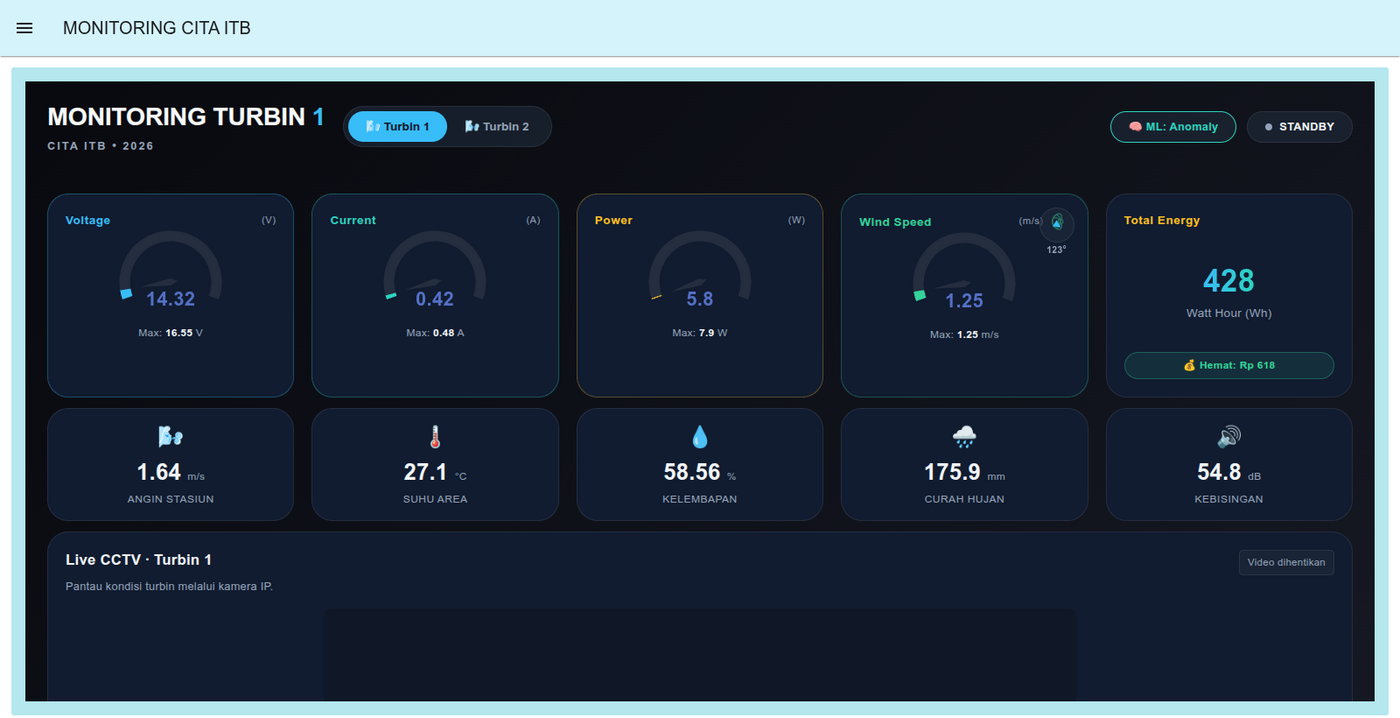
\includegraphics[width=0.92\linewidth]{../presentasi/gambar/hmi-dashboard-2026-10-20.png}
\caption{Dashboard HMI Node-RED (\url{http://citaitb.com:1880/dashboard}, juga lewat IP \cmd{103.102.153.154}), data live 20 Okt 2026 pukul 19.11 WIB.
Halaman \emph{Analys} (\cmd{/dashboard/kontrol}) dan \emph{About \& Spesifikasi} (\cmd{/dashboard/about}) belum berisi widget.}
\end{figure}

\section{Pipeline data dan fitur}
\subsection{Preprocessing}
\begin{figure}[h]
\centering\resizebox{\linewidth}{!}{\diagram{pipeline}}
\caption{Alur \cmd{ml/common/preprocess.py}. Angka = hasil eksekusi 20 Okt.}
\end{figure}

\subsection{Data eksternal}
\begin{itemize}
  \item \textbf{Open-Meteo} (gratis, tanpa API key, CC BY 4.0): \emph{arsip prakiraan} per jam untuk titik $-6{,}891$; $107{,}610$, berisi angin
        10/80/120 m, hembusan, arah, suhu, kelembapan, tekanan, dan awan. Karena ini arsip keluaran model prakiraan, fiturnya tersedia juga saat operasi nyata,
        jadi tidak ada kebocoran. Korelasi dengan angin stasiun per jam hanya 0,14, karena atap kota bersifat turbulen dan grid model kasar.
        Model memakai data ini sebagai konteks; model tanpa data luar juga diuji (mode offline).
  \item \textbf{BMKG} (\cmd{adm4} \cmd{32.73.02.1006} = Lebak Siliwangi, Coblong, terkonfirmasi dari respons API): tidak punya arsip, sehingga
        \cmd{ml/common/fetch\_bmkg.py} sudah merekam dan perlu dijalankan tiap 3 jam (cron).
\end{itemize}

\subsection{Fitur dan target}
\begin{figure}[h]
\centering\resizebox{0.9\linewidth}{!}{\diagram{jendela}}
\caption{Fitur hanya memakai data sampai waktu $t$; target = rata-rata daya 60 menit berikutnya (= energi jam depan).}
\end{figure}
16 fitur (urutan = urutan byte ke FPGA): \cmd{p\_now}, \cmd{p\_lag5}, \cmd{p\_lag15}, \cmd{p\_lag30}, \cmd{p\_lag60}, \cmd{p\_mean60},
\cmd{w\_now}, \cmd{w\_mean10}, \cmd{w\_mean60}, \cmd{w3\_mean10}, \cmd{dir\_sin}, \cmd{dir\_cos}, \cmd{hour\_sin}, \cmd{hour\_cos}, \cmd{rho}, \cmd{om\_wind\_next}.
Sampel yang jendelanya ($t-60\ldots t+60$) melewati celah $>$10 menit dibuang. Split kronologis:
\textbf{latih} 30 Mar--31 Jul (99.260 sampel), \textbf{validasi} Agu--Sep (31.700), \textbf{uji} 1--20 Okt (16.255).

\section{Fitur 2: prediksi rata-rata daya 1 jam ke depan}
\subsection{Hasil perbandingan metode}
Semua metode memakai fitur, split, dan data uji yang sama. Skill = $1 - \mathrm{RMSE}/\mathrm{RMSE}_\text{persistence}$.

\IfFileExists{../presentasi/data/tabel_benchmark.tex}{\begin{small}
\begin{longtable}{@{}r p{6.2cm} p{3.4cm} r r r p{2.6cm}@{}}
\toprule
\# & Metode & Kelompok & MAE (W) & RMSE (W) & Skill & FPGA MAC4 \\ \midrule \endhead
1 & Transformer (riwayat 60 menit) & Jaringan saraf (sekuensial) & 5,70 & 10,07 & +0,411 & sulit (softmax, memori besar) \\
2 & Regresi linear & Linear & 5,71 & 10,23 & +0,402 & ya \\
3 & Ridge & Linear & 5,71 & 10,23 & +0,402 & ya \\
4 & TCN (riwayat 60 menit) & Jaringan saraf (sekuensial) & 5,46 & 10,25 & +0,401 & mungkin (konvolusi) \\
5 & MLP float 16-8-1 & Jaringan saraf (tabular) & 5,59 & 10,25 & +0,401 & ya, bila FSM diubah \\
6 & \textbf{MLP INT8 (QAT, identik RTL)} & Varian hardware (INT8) & 5,48 & 10,25 & +0,401 & ya (bobot ini) \\
7 & Lasso & Linear & 5,71 & 10,25 & +0,401 & ya \\
8 & ElasticNet & Linear & 5,70 & 10,25 & +0,401 & ya \\
9 & LSTM (riwayat 60 menit) & Jaringan saraf (sekuensial) & 5,59 & 10,35 & +0,395 & sulit (sigmoid/tanh, sekuensial) \\
10 & GRU (riwayat 60 menit) & Jaringan saraf (sekuensial) & 5,54 & 10,41 & +0,392 & sulit (sigmoid/tanh, sekuensial) \\
11 & MLP float 16-16-1 & Jaringan saraf (tabular) & 5,67 & 10,41 & +0,392 & ya, bila FSM diubah \\
12 & MLP float 16-32-16-1 (acuan QAT, train\_mlp.py) & Varian hardware (INT8) & 5,59 & 10,44 & +0,390 & ya \\
13 & CNN 1D (riwayat 60 menit) & Jaringan saraf (sekuensial) & 5,60 & 10,46 & +0,389 & mungkin (MAC sama, FSM lebih rumit) \\
14 & MLP float 16-32-16-1 & Jaringan saraf (tabular) & 5,62 & 10,47 & +0,388 & ya (16-32-16-1 = RTL sekarang) \\
15 & MLP float 16-64-32-1 & Jaringan saraf (tabular) & 5,64 & 10,49 & +0,387 & ya, bila FSM diubah \\
16 & ExtraTrees & Pohon & 5,46 & 10,59 & +0,382 & tidak \\
17 & KNN (k=25) & Kernel/tetangga & 5,52 & 10,62 & +0,380 & tidak \\
18 & MLP INT8 (PTQ: dibulatkan tanpa QAT) & Varian hardware (INT8) & 6,75 & 10,65 & +0,378 & ya (bobot ini) \\
19 & ARIMA(2,0,1) deret 10 menit* & Statistik & 6,19 & 10,77 & +0,391 & ya (kecil) \\
20 & Polinomial derajat 2 + Ridge & Linear & 5,89 & 10,87 & +0,365 & ya \\
21 & Random Forest & Pohon & 5,74 & 10,91 & +0,363 & tidak \\
22 & campuran mean60 + klimatologi (a=0.35) & Baseline & 5,91 & 11,00 & +0,357 & tidak perlu \\
23 & LightGBM tanpa Open-Meteo (offline) & Varian data & 5,76 & 11,03 & +0,355 & tidak \\
24 & LightGBM kuantil P50 (+ interval P10–P90) & Probabilistik & 5,64 & 11,12 & +0,350 & tidak \\
25 & LightGBM & Pohon & 5,79 & 11,16 & +0,348 & tidak \\
26 & SVR RBF (15 rb sampel) & Kernel/tetangga & 5,65 & 11,23 & +0,344 & tidak \\
27 & HistGradientBoosting & Pohon & 5,82 & 11,27 & +0,341 & tidak \\
28 & XGBoost & Pohon & 5,98 & 11,40 & +0,334 & tidak \\
29 & CatBoost & Pohon & 5,91 & 11,47 & +0,330 & tidak \\
30 & Decision Tree & Pohon & 6,20 & 11,58 & +0,323 & tidak \\
31 & Kurva daya $\times$ angin 60 menit terakhir & Fisika & 7,06 & 12,38 & +0,277 & tabel di ESP32 \\
32 & smart persistence (rata-rata 60 menit terakhir) & Baseline & 7,12 & 12,62 & +0,262 & tidak perlu \\
33 & klimatologi per jam & Baseline & 6,85 & 12,89 & +0,247 & tidak perlu \\
34 & moving average 10 menit & Baseline & 7,47 & 14,39 & +0,159 & tidak perlu \\
35 & persistence (P sekarang) & Baseline & 8,67 & 17,11 & +0,000 & tidak perlu \\
36 & Kurva daya $\times$ prakiraan Open-Meteo & Fisika & 11,45 & 17,19 & -0,005 & tabel di ESP32 \\
\bottomrule
\end{longtable}
\end{small}}{\tbd{tabel benchmark}}

\IfFileExists{../presentasi/data/benchmark_ringkas.tex}{\textbf{Ringkasan.} 36 metode diuji. Terbaik: \textbf{Transformer (riwayat 60 menit)} (RMSE 10,07 W, skill +0,411). Baseline terbaik: campuran mean60 + klimatologi (a=0.35) (11,00 W). Model yang benar-benar berjalan di FPGA, \textbf{MLP INT8 (QAT)}, ada di peringkat 6 (RMSE 10,25 W): selisihnya dengan model terbaik adalah harga yang dibayar untuk 1.040 MAC INT8, tanpa sistem operasi, dan hasil yang dapat diverifikasi bit per bit.}{}

\IfFileExists{../presentasi/data/contoh_prediksi.csv}{%
\begin{figure}[h]
\centering
\begin{tikzpicture}
\begin{axis}[width=\linewidth, height=5.4cm, xlabel={jam sejak 00.00 WIB, \input{../presentasi/data/contoh_prediksi_tanggal.txt}}, ylabel={daya rata-rata 1 jam ke depan (W)},
             ymin=0, xmin=0, xmax=48, xtick={0,6,...,48}, tick label style={font=\scriptsize}, label style={font=\scriptsize},
             legend style={font=\scriptsize, at={(0.99,0.98)}, anchor=north east}, legend columns=2]
  \addplot[name path=lo, draw=none, forget plot] table[col sep=comma, x=jam, y=p10] {\datafile{contoh_prediksi.csv}};
  \addplot[name path=hi, draw=none, forget plot] table[col sep=comma, x=jam, y=p90] {\datafile{contoh_prediksi.csv}};
  \addplot[izma!15, forget plot] fill between[of=lo and hi];
  \addplot[black, thick] table[col sep=comma, x=jam, y=aktual] {\datafile{contoh_prediksi.csv}};
  \addplot[lama, dashed] table[col sep=comma, x=jam, y=persistence] {\datafile{contoh_prediksi.csv}};
  \addplot[izma, thick] table[col sep=comma, x=jam, y=int8] {\datafile{contoh_prediksi.csv}};
  \legend{aktual, persistence, MLP INT8 (FPGA)}
\end{axis}
\end{tikzpicture}
\caption{Contoh dua hari di data uji (hari dengan energi terbesar). Area biru muda = interval P10--P90 dari model kuantil.}
\end{figure}}{}

\subsection{Mengapa lebih maju dari yang sudah ada di PLN}
\begin{enumerate}
  \item \textbf{Berjalan di edge, tanpa internet}: INT8 di FPGA atau ESP32. Data dan prediksi tetap ada saat internet mati (masalah nyata: 2.787 reboot).
  \item \textbf{Interval ketidakpastian} (P10--P90), bukan satu angka, sehingga keputusan isi baterai/ambil PLN bisa memperhitungkan risiko.
  \item \textbf{Terhubung ke hardware}: akurasi, siklus, dan energi per prediksi diukur untuk model yang sama persis (bit-exact).
  \item \textbf{Rantai sampai baterai/AC} (fitur 3), yaitu bagian yang menurut PLN belum ada.
\end{enumerate}

\section{Hubungan ML dan FPGA}\label{sec:fpga}
\begin{figure}[h]
\centering\resizebox{0.95\linewidth}{!}{\diagram{fpga_alur}}
\caption{Model dilatih langsung dalam aritmetika bilangan bulat RTL (quantization-aware training), sehingga tidak ada tahap konversi yang bisa menggeser hasil.}
\end{figure}
\begin{figure}[h]
\centering\resizebox{0.95\linewidth}{!}{\diagram{mac4}}
\caption{Datapath akselerator (RTL Alif, \cmd{feature/fpga}). Satu prediksi = 260 langkah MAC4 + pasca-proses = 309 siklus di RTL Verilog (cermin Python menghitung 310), $\approx$11,4\,$\mu$s pada 27 MHz.}
\end{figure}
\begin{center}
\begin{tabular}{@{}l r r r@{}}
\toprule
Sumber daya Tang Nano 4K (GW1NSR-4C) & Terpakai & Kapasitas & \% \\
\midrule
LUT4 & 1.126 & 4.608 & 24 \\
Flip-flop & 733 & 3.456 & 21 \\
BSRAM (bobot) & 2 & 10 & 20 \\
Pengali MULT9X9 & 4 & 32 & 12 \\
\midrule
Fmax setelah routing & \multicolumn{3}{r}{85,7 MHz (target 27 MHz, margin 3,2$\times$)} \\
Siklus per prediksi (iverilog) & \multicolumn{3}{r}{309 $\approx$ 11,4\,$\mu$s pada 27 MHz} \\
\bottomrule
\end{tabular}
\end{center}
\begin{figure}[h]
\centering\resizebox{\linewidth}{!}{\diagram{verifikasi}}
\caption{Status verifikasi dari model sampai papan dan dashboard (21 Okt): semua tahap selesai.}\label{fig:verif}
\end{figure}
\begin{itemize}
  \item \textbf{Verifikasi bertahap (Gambar~\ref{fig:verif}):} PyTorch-QAT = integer numpy (16.255 sampel) = golden model = cermin RTL Python (597 vektor)
        = \textbf{RTL Verilog di iverilog}: core \cmd{top.v} 2.000 vektor acak + 597 vektor data nyata, SoC lewat UART 16 + 50 vektor, setiap neuron
        h1/h2, keluaran, dan jumlah siklus (309) sama persis. Skrip: \cmd{hw/sim/run\_regression.py} dan \cmd{run\_regression\_real.py} (branch \cmd{feature/integrasi}).
  \item \textbf{Papan Tang Nano 4K:} bitstream dibangun dengan toolchain open-source (OSS CAD Suite: yosys + nextpnr-himbaechel + gowin\_pack),
        bobot hasil training ditanam di BSRAM, lalu di-flash ke SRAM dengan \cmd{openFPGALoader} (CRC sukses). Papan harus dicolok langsung ke laptop:
        lewat hub USB bertingkat, transfer JTAG gagal.
  \item \textbf{Uji HIL di papan (21 Okt):} ESP32-S3 tersambung langsung ke pin header 44/46 (bank 1, diukur 3,3 V; pin 44 dan 46 di bank yang sama menurut chipdb).
        Bitstream RTL 21 Okt dengan bobot hasil latih dimuat lalu ditulis ke flash. Firmware \cmd{esp32s3\_hil} mengirim 597 vektor uji nyata per ronde:
        \textbf{5.373/5.373 inferensi identik} dengan golden model dan MLP di CPU ESP32 (9 ronde), 309 siklus, pulang-pergi 482\,$\mu$s, tanpa paket hilang atau CRC salah
        (\cmd{docs/demo/hil-2026-10-21.txt}). UART akselerator memang tidak lewat USB bawaan papan, sesuai skematik.
  \item \textbf{Live:} firmware \cmd{esp32s3\_bridge} membuat ESP32-S3 mengambil 16 fitur dari \cmd{WEC/prediksi} (MQTT, lewat hotspot), meneruskannya ke FPGA, lalu mengirim \cmd{WEC/fpga};
        sejak 21 Okt 11.56 dashboard menampilkan ``Chip: Tang Nano 4K aktif'' dan hasil chip selalu sama dengan CPU.
  \item \textbf{Temuan untuk RTL:} karena M=32/S=8 dikunci untuk semua lapisan, bobot hasil latih hanya memakai rentang $\pm5$ dari $\pm127$ (3 bit).
        Akurasi tetap mengalahkan baseline. Uji 21 Okt (\cmd{eksperimen\_ms\_per\_lapisan.py}): M per lapisan memakai rentang bobot sampai $\pm45$, tetapi MAE uji tetap 5,45--5,65 W untuk 7 kombinasi (sebesar selisih antar-pelatihan), jadi bukan prioritas RTL.
  \item \textbf{UART:} RTL 21 Okt (Alif) memakai paket berbingkai 19 B \cmd{[AA 55, 16 fitur, CRC-8]} $\to$ 7 B \cmd{[55 AA, status, prediksi, siklus, CRC-8]}, 921600 bps, dengan watchdog. \cmd{docs/kontrak-uart.md} sudah diperbarui mengikuti RTL, dan firmware ESP32 memakai format ini (batas waktu 20 ms, pemulihan sinkron).
  \item File untuk Alif dan Genis: \cmd{ml/forecast/model/export/} berisi \cmd{weights.hex}, \cmd{weights32.hex}, \cmd{bias.hex}, \cmd{test\_vectors.csv},
        \cmd{mlp\_int8.h}, dan \cmd{mlp\_float\_int8.tflite}. Skala tiap fitur ada di \cmd{docs/kontrak-kuantisasi.md}.
\end{itemize}

\section{Fitur 1: status turbin}
\begin{center}
\small
\begin{tabularx}{\linewidth}{@{}X r@{}}
\toprule
Percobaan & Hasil \\
\midrule
Reproduksi TA (Cp, D=3 m, $\rho$=1,156, angin Arduino, 5.000/kelas, split acak, SVM RBF) & akurasi 97,6\% (TA: 98,22\%) \\
Model asli dari Raspi pada split uji yang sama & 97,8\% \\
Model asli pada data 16 Jun--20 Okt (belum pernah dilihat) & 98,2\% (tebak kelas terbanyak: 51,9\%) \\
Versi perbaikan (angin stasiun, D=2,5 m, $\rho$ dari data, kronologis): SVM RBF / RF / LightGBM / SVM linear & 99,1 / 98,8 / 98,7 / 90,5\% \\
\bottomrule
\end{tabularx}
\end{center}
\textbf{Catatan jujur.} Label Cp dihitung langsung dari V, I, dan $v$, sehingga model hanya meniru rumus (aturan Cp langsung = 100\%).
Dengan angin Arduino macet di 1,25 m/s (42\% data), kelas \emph{Anomaly} pada data TA sebagian besar mencerminkan sensor rusak, bukan turbin rusak.

\textbf{Pendekatan baru (\cmd{anomaly.py}).} Model kuantil mempelajari daya \emph{wajar} untuk kondisi angin, lalu membandingkannya dengan daya aktual
(rasio 30 menit, ambang dikalibrasi di Agu--Sep untuk alarm palsu $\approx$1\%). Uji dengan kerusakan buatan di data Okt:
\begin{itemize}
  \item daya tersisa 20\%: terdeteksi 68\% jendela (alarm palsu 3,8\%); tersisa 40\%: 25\%; degradasi ringan (60--80\%) belum terdeteksi;
  \item aturan Cp $<$ 0,10 (gaya TA) dan Isolation Forest: hampir tidak mendeteksi apa pun;
  \item jendela 2--6 jam: alarm palsu tinggi karena perilaku Okt bergeser dari Agu--Sep, sehingga ambang perlu dikalibrasi ulang berkala di lapangan.
\end{itemize}
Keterbatasannya ada pada sensor: satu anemometer di atap turbulen membuat hubungan angin--daya per menit sangat berisik.

\subsection{Versi INT8 untuk chip}\label{sec:f1int8}
Model kuantil diganti \textbf{MLP kurva daya wajar} dengan topologi dan aritmetika yang sama dengan fitur 2 (16-32-16-1, requantize $(acc\cdot32)\gg8$),
sehingga satu akselerator bisa menjalankan keduanya (usulan: \cmd{docs/usulan-rtl-dua-model.md}). Masukan 16 fitur angin/cuaca (tanpa daya), target rata-rata daya 10 menit.
\begin{itemize}
  \item Uji Okt: MAE 2,57 W, RMSE 5,93 W; PyTorch QAT = integer: 0 beda. Bobot lulus RTL Verilog yang ada (600 vektor nyata + 2.000 acak, 309 siklus).
  \item Status = rasio aktual/wajar rata-rata 30 menit: $<$0,42 di bawah normal, $>$1,463 di atas normal (cek sensor), daya wajar $\le$5 W = angin lemah.
  \item Uji kerusakan buatan: daya tersisa 20\% terdeteksi 67,5\% jendela (alarm palsu 4,0\%); 40\%: 10\%; 60\%: 7,5\%.
  \item \textbf{Kegunaan kedua:} saat PZEM diam, daya wajar ini menggantikan fitur daya pada prediksi 1 jam (\S\ref{sec:dash}).
\end{itemize}

\section{Fitur 3: setelah inverter dan ke baterai}
\begin{figure}[h]
\centering\resizebox{0.85\linewidth}{!}{\diagram{baterai}}
\caption{Sistem sekarang (atas) dan usulan (bawah). Tulisan merah = sensor yang harus ditambahkan.}
\end{figure}
Data yang \textbf{harus diukur sendiri} (tidak ada API karena spesifik lokasi):
\begin{itemize}
  \item V/I baterai, SoC (BMS), dan suhu baterai;
  \item V/I/P/PF keluaran inverter;
  \item energi ke dump load;
  \item konsumsi beban.
\end{itemize}
Yang bisa dari \textbf{sumber publik}:
\begin{itemize}
  \item kurva efisiensi inverter (database CEC/Sandia lewat pvlib);
  \item dataset baterai NASA PCoE dan CALCE untuk estimator SoC/SoH;
  \item prakiraan cuaca (Open-Meteo, BMKG).
\end{itemize}
Rinciannya ada di \cmd{docs/kajian-inverter-baterai.md}.

\IfFileExists{../presentasi/data/tabel_baterai.tex}{\begin{center}\small
\begin{tabular}{@{}l r r r r@{}}
\toprule
Prediksi daya DC yang dipakai & MAE SoC 1 jam (poin \%) & MAE energi ke baterai (Wh) & Presisi impor PLN & Recall \\ \midrule
persistence & 1,82 & 10,54 & 0,94 & 0,93 \\
smart persistence & 1,51 & 9,01 & 0,95 & 0,97 \\
MLP INT8 (FPGA) & 1,12 & 7,66 & 0,96 & 0,93 \\
LightGBM & 1,22 & 7,76 & 0,96 & 0,92 \\
Ideal (daya DC aktual) & 0,12 & 3,49 & 1,00 & 0,95 \\
\bottomrule
\end{tabular}
\end{center}
Simulasi 1--20 Okt: energi turbin 4706,80 Wh, beban 5139,50 Wh, dibuang 56,00 Wh, impor PLN 1278,20 Wh; SoC di batas minimum 29,50\% waktu.}{\tbd{hasil simulasi baterai}}

\IfFileExists{../presentasi/data/soc_3hari.csv}{%
\begin{figure}[h]
\centering
\begin{tikzpicture}
\begin{axis}[width=0.9\linewidth, height=4.2cm, xlabel={jam sejak 1 Okt 07.00 WIB}, ylabel={SoC (\%)}, ymin=0, ymax=105, xmin=0, xmax=72,
             xtick={0,12,...,72}, tick label style={font=\scriptsize}, label style={font=\scriptsize}]
  \addplot[genis, thick] table[col sep=comma, x=jam, y=soc] {\datafile{soc_3hari.csv}};
  \addplot[merah, dashed, domain=0:72] {10};
\end{axis}
\end{tikzpicture}
\caption{Simulasi SoC baterai 384 Wh selama 3 hari pertama Okt dengan daya turbin terukur dan beban 6 W + 25 W malam (skenario defisit). Garis merah = batas 10\% (ambil dari PLN).}
\end{figure}}{}

\textbf{Membaca tabel:} galat SoC 1 jam adalah ukuran utama; MLP INT8 paling kecil di antara model yang bisa dipakai. Presisi/recall impor PLN tinggi untuk semua metode (termasuk persistence) karena sebagian besar kejadian terjadi saat SoC sudah di batas minimum, sehingga metrik ini kurang membedakan metode.

\textbf{Catatan:} dengan baterai, titik kerja turbin berubah (tegangan dijepit baterai/MPPT), sehingga model daya perlu dilatih ulang
dengan data setelah baterai terpasang. Semua angka di bagian ini adalah simulasi dengan asumsi yang tertulis di \cmd{ml/battery/sim\_battery.py}.


\section{Edge node ESP32-S3}\label{sec:esp32}
Firmware PlatformIO di \cmd{edge/esp32/} untuk papan tim \textbf{ESP32-S3-DevKitC-1 N16R8} (dan ESP32 klasik). Inti perhitungan (\cmd{lib/wec\_core}) ditulis C++ murni
sehingga bisa diuji di laptop dengan data rujukan yang sama dengan mesin Node-RED.
\begin{center}
\small
\begin{tabularx}{\linewidth}{@{}l X@{}}
\toprule
Tiap 3 detik & PZEM-017 (input reg.\ 0--5, 9600 8N2) + stasiun (0x01F4--0x01FA, 0x0201, 4800 8N1) di satu bus RS-485; anemometer optik lewat interupsi; kirim \cmd{TurbinAnginESP/*} format Raspi \\
Tiap menit & agregat 1 menit $\to$ 16 fitur INT8 $\to$ FPGA (19 B $\to$ 7 B + CRC-8, 921600 bps, batas 20 ms) atau MLP yang sama di CPU; status kurva daya; SoC + relai PLN/dump load (histeresis); \cmd{WEC/esp32/*} \\
Offline & MQTT putus $\to$ antrean LittleFS (maks 600 KB, $\pm$2 hari) dikirim ulang saat tersambung; Open-Meteo sekali ambil berlaku 3 hari \\
\bottomrule
\end{tabularx}
\end{center}
Hasil uji inti (\cmd{python3 edge/esp32/test/run\_native.py}): MLP dua model vs test vector golden 0 beda (597 + 600, termasuk h1/h2); kuantisasi 0 beda (400);
32 fitur dari riwayat per menit vs Python 0 beda (400), input INT8 identik 400/400; baterai vs \cmd{engine\_core.js} 0 beda (2.000 kasus).
Build \cmd{esp32s3}: RAM 32\% (106 KB), flash 13\% dari 16 MB. UART ke FPGA sudah diuji di papan (HIL, \S\ref{sec:fpga}). \textbf{Belum diuji di papan}: Modbus, interupsi anemometer, dan relai.
Ditemukan dan diperbaiki saat porting: header \cmd{mlp\_int8.h} memuat literal \cmd{0f} yang tidak sah di C (sekarang \cmd{0.0f}). Mode cadangan PZEM diam juga ada di firmware (daya wajar dari MLP kurva daya), dan fiturnya sama dengan \cmd{engine\_core.js} (120 menit uji, separuh menit dayanya dikosongkan, 0 beda).

\textbf{Jembatan demo sebelum ESP32 dirakit.} Mesin ML mengirim \cmd{xq} (16 fitur INT8) di \cmd{WEC/prediksi}; \cmd{fpga\_bridge.py} di laptop membungkusnya menjadi paket 19 byte + CRC-8 ke FPGA lewat USB-TTL 921600 bps (TXD$\to$44, RXD$\leftarrow$46), menerima 7 byte, membandingkan dengan hasil CPU, lalu mengirim \cmd{WEC/fpga}. Dashboard menampilkan baris \emph{Chip} (sumber, siklus, waktu pulang-pergi, identik/beda) dan InfluxDB menyimpannya (\cmd{wec\_fpga}). Tanpa papan, \cmd{--sim} memakai golden model dan ditandai ``simulasi''.

\section{Dashboard hackathon dan mesin ML di Node-RED}\label{sec:dash}
\begingroup\sloppy
\begin{itemize}
  \item \textbf{Halaman:} \url{http://citaitb.com:1880/dashboard/hackathon} (dulu \cmd{/v2}). Dibangun dari template Genis lewat \cmd{patch\_template.py} + \cmd{skin\_hackathon.py};
        template Genis di \cmd{/dashboard/dashboard} identik dengan aslinya. Deploy: \cmd{dashboard/wec/deploy.py} (backup dulu, mode \emph{nodes}).
  \item \textbf{Mesin ML} (function node, logika = Python): tiap menit membuat prediksi 1 jam + P10--P90, status kurva daya, dan SoC baterai; hasil ke dashboard dan MQTT \cmd{WEC/*}.
  \item \textbf{Penyebab ``menunggu'' dan perbaikannya.} (1) Model butuh 50 dari 60 menit data daya; saat PZEM diam, daya kosong diganti daya wajar dari MLP kurva daya
        (label \emph{mode cadangan}). (2) Riwayat hanya di memori, hilang tiap deploy: kini snapshot 240 menit dikirim ke \cmd{WEC/state} (retained, $\pm$13 KB) tiap 5 menit dan dipulihkan saat start.
        (3) Alasan ditampilkan: PZEM tidak merespons, stasiun cuaca diam, atau tidak ada data sejak jam tertentu.
        (4) \textbf{Data berlubang} (Raspi reboot 07.00, 07.10, 07.40 pada 21 Okt): syarat ketat 50 dari 60 menit hampir tidak pernah terpenuhi. Mode \emph{celah} menurunkan syarat ke separuh jendela dan mencari lag sampai 5 menit ke belakang, hanya bila syarat ketat gagal. Status juga disimpan di flow context sehingga deploy tidak menghapus riwayat.
\end{itemize}
\endgroup
\begin{center}
\small
\begin{tabularx}{0.8\linewidth}{@{}X r r@{}}
\toprule
Uji 1--20 Okt (prediksi rata-rata daya 1 jam) & MAE (W) & menit \\
\midrule
Mode normal (daya PZEM) & 4,76 & 11.166 \\
Mode cadangan (PZEM diam, daya dari angin) & 4,72 & 11.166 \\
Persistence (butuh PZEM) & 6,88 & 11.166 \\
\midrule
Cek offline Python: normal / cadangan / persistence & 5,41 / 5,42 / 8,48 & 10.946 \\
\midrule
Data berlubang 20\% (4 menit hilang tiap 10--30 menit): mode celah / utuh / persistence & 5,07 / 5,00 / 7,16 & 19.582 \\
Cakupan prediksi saat data berlubang: tanpa / dengan mode celah & 12,5\% / 97,7\% & \\
\bottomrule
\end{tabularx}
\end{center}
{\small Simulasi lengkap function node (\cmd{test\_tanpa\_pzem.js}) dan cek offline (\cmd{ml/forecast/eval\_tanpa\_pzem.py}) memakai himpunan menit yang berbeda, sehingga angkanya tidak sama; keduanya menunjukkan mode cadangan setara mode normal.}

\section{Database InfluxDB}\label{sec:influx}
InfluxDB 2.7 di laptop (\cmd{127.0.0.1:8086}), berjalan paralel dengan Google Sheets. Isi: \cmd{turbin\_1min} (181.228 menit historis), hasil uji ML 1--20 Okt,
simulasi baterai, data live MQTT (\cmd{TurbinAngin/\#}, \cmd{TurbinAnginESP/\#}, \cmd{WEC/\#}). Dashboard 11 panel; MAE di Flux sama dengan Python
(MLP INT8 5,48 W, Transformer 5,70 W, persistence 8,67 W). Perbaikan 21 Okt: Raspi mengirim \cmd{voltage/current/power/energy} huruf kecil sehingga tersimpan sebagai
\cmd{power} (bukan \cmd{power\_w}); subscriber diperbaiki dan 44 titik lama disalin dengan nama yang benar.

\section{Model bisnis dan substitusi impor}\label{sec:bisnis}
\textbf{Segmen:} pengelola PLTB/PLTH kecil dan pembangkit tersebar (off-grid, hibrida, kampus, BTS); integrator EBT dan BUMN energi; PLN Puslitbang sebagai mitra pilot.
\textbf{Pendapatan}, diurutkan sesuai tahap validasi: pilot + jasa integrasi; modul per turbin + dukungan tahunan; lisensi IP core ke OEM/mitra semikonduktor.
Harga belum dikunci sebelum 5--8 wawancara calon pengguna (rencana di \cmd{docs/business/draf-bmc-bootcamp.pptx}).
\begin{center}
\small
\begin{tabularx}{0.85\linewidth}{@{}X r@{}}
\toprule
Komponen inti per turbin (harga RAB, Tokopedia, Okt 2026) & Harga \\
\midrule
ESP32-S3-DevKitC-1 N16R8 & Rp144.900 \\
Modul RS-485 ke TTL terisolasi & Rp139.125 \\
Tang Nano 4K (perkiraan, belum ada di RAB; ritel luar negeri US\$18--21) & $\pm$Rp300.000 \\
PCB carrier 2 lapis (1/3 paket cetak lokal Rp119.700) & Rp39.900 \\
\midrule
\textbf{Edge node} & \textbf{$\approx$Rp624.000} \\
Pembanding gateway SBC: Orange Pi 3B 8 GB + microSD + casing + adaptor (RAB) & Rp3.294.795 \\
\bottomrule
\end{tabularx}
\end{center}
\textbf{Strategi substitusi impor dan TKDN (bertahap):}
\begin{itemize}
  \item \emph{Sekarang:} IP core akselerator (RTL), golden model, firmware, model ML, pipeline data, dan dashboard dirancang sendiri; papan pengembangan masih impor.
  \item \emph{Produk:} PCB carrier rancangan sendiri dirakit EMS lokal, panel dan kabel dari pasar lokal, server sendiri (Node-RED/InfluxDB) alih-alih layanan cloud asing.
  \item \emph{Lanjutan:} IP core yang sama dibawa ke ASIC (OpenLane/SKY130 lewat MPW) untuk menggantikan SBC/NPU impor; persentase TKDN dihitung setelah BOM produk final.
\end{itemize}

\section{Pembaruan 21 Okt sore: model offline, M per lapisan, daya komputasi}\label{sec:v3}
\textbf{Model INT8 offline.} Bila internet putus lebih dari 3 hari, prakiraan Open-Meteo habis dan model utama tidak bisa dihitung. Model offline memakai
topologi, aritmetika RTL, dan skala fitur yang sama, dengan masukan ke-16 (\cmd{om\_wind\_next}) selalu 0, sehingga kontrak UART tidak berubah
(\cmd{ml/forecast/train\_mlp\_offline.py}; PyTorch = integer 0 beda; C++ = golden 1.097 vektor 0 beda).
\begin{center}
\small
\begin{tabularx}{0.85\linewidth}{@{}X r r@{}}
\toprule
Uji 1--20 Okt (16.255 menit sama) & MAE (W) & RMSE (W) \\
\midrule
Model utama (dengan Open-Meteo) & 5,48 & 10,25 \\
\textbf{Model offline (tanpa Open-Meteo)} & \textbf{5,62} & \textbf{10,18} \\
Model utama dengan masukan ke-16 = 0 (tanpa model offline) & 5,73 & 10,98 \\
Persistence & 8,67 & 17,11 \\
\bottomrule
\end{tabularx}
\end{center}
Node-RED dan firmware ESP32 memakainya otomatis (label ``offline''); karena FPGA berisi bobot model utama, mode offline dihitung di CPU dan
\cmd{WEC/prediksi} tidak membawa \cmd{out\_q} agar perbandingan chip tetap adil.

\textbf{M requantize per lapisan (usulan RTL lama).} Tujuh kombinasi M per lapisan (S = 8) dilatih ulang dengan QAT yang sama
(\cmd{ml/forecast/eksperimen\_ms\_per\_lapisan.py}): rentang bobot naik dari $\pm6$ sampai $\pm45$, tetapi MAE uji tetap 5,45--5,65 W dan RMSE
10,12--10,46 W, sebesar selisih antar-pelatihan dengan konfigurasi yang sama (model resmi 5,48 W, latih ulang 5,65 W). Kesimpulan: RTL tidak perlu diubah.

\textbf{Pengukur daya komputasi.} ESP32 klasik (\cmd{edge/esp32}, env \cmd{esp32\_daya}) membaca INA1 = Raspberry Pi (I2C 21/22) dan INA2 = Tang Nano 4K + ESP32-S3
(I2C 18/19), kalibrasi 32V\_2A, lalu mengirim \cmd{WEC/daya} tiap detik; Node-RED meneruskannya ke panel ``Konsumsi Daya'', InfluxDB mencatat \cmd{wec\_daya}.
Kedua ESP32 tersambung lewat eduroam (WPA2-Enterprise, akun hanya di \cmd{secrets.h}) dengan cadangan hotspot. Status 21 Okt: data sampai ke dashboard,
pembacaan masih 0 V/0 A karena catu belum dilewatkan Vin+/Vin$-$; diagram pemasangan di \cmd{docs/demo/pemasangan-ina219.png}.

\textbf{Temuan keamanan (untuk pengelola server/Genis).}
\begin{itemize}
  \item Sandi cetak PDF di template dashboard Genis diperiksa di browser, sehingga terbaca oleh siapa pun yang membuka halaman.
  \item Port MySQL 3306 di server \cmd{citaitb.com} terbuka ke internet; sebaiknya dibatasi firewall.
  \item Raspi tersambung eduroam dengan akun kampus pribadi; sebaiknya akun khusus perangkat.
\end{itemize}

\section{Rencana dan risiko}
\begin{center}
\begin{tikzpicture}[x=1.5cm, y=0.55cm, every node/.style={font=\scriptsize}]
  \foreach \i/\d in {0/20 Okt, 1/21 Okt, 2/22 Okt, 3/23 Okt, 4/Nov--Des}{\node at (\i+0.5,6.6) {\textbf{\d}}; \draw[black!20] (\i,0) -- (\i,6.3);}
  \draw[black!20] (5,0) -- (5,6.3);
  \foreach \y/\t/\a/\b/\c in {6/Data + fitur 1--3 (hari ini)/0/1/izma, 5/Integrasi INT8 ke ESP32 + FPGA/1/2.5/alif, 4/Dashboard prediksi + replay/1/2.5/genis,
                               3/Ukur energi per prediksi/1.5/2.7/shania, 2/Laporan v2 + deck final/2/3/izma, 1/Pitching juri/3/4/shania,
                               0/Uji lapangan + data baterai/4/5/lama}
    {\fill[\c!55] (\a,\y-0.35) rectangle (\b,\y+0.35); \node[anchor=east] at (0,\y) {\t};}
\end{tikzpicture}
\end{center}
\begin{center}
\small
\begin{tabularx}{\linewidth}{@{}X X@{}}
\toprule
Risiko & Mitigasi \\
\midrule
Jembatan ESP32-S3 butuh hotspot HP saat demo & bila WiFi gagal, \cmd{fpga\_bridge.py --sim} di laptop (ditandai simulasi); HIL sudah lulus di papan \\
Papan FPGA/ESP32 bermasalah saat demo & \cmd{mlp\_int8.h} bit-exact di ESP32; demo simulasi fungsional diizinkan panitia \\
PZEM tidak merespons / Raspi reboot saat demo & mode cadangan (daya dari angin) + snapshot riwayat; data historis di InfluxDB \\
Data Mei--Okt sebagian rusak & sudah direkonstruksi dari V$\times$I; ekspor ulang dari Sheets akan menggantikan \\
Internet di lokasi tidak stabil & buffer lokal di ESP32 + mode offline (tanpa Open-Meteo) \\
\bottomrule
\end{tabularx}
\end{center}

% ======================================================================
\clearpage
\part*{Bagian II --- User guide: sistem monitoring dari awal sampai akhir}
\addcontentsline{toc}{part}{Bagian II --- User guide}

Panduan ini untuk anggota tim yang perlu membuka Raspi turbin, memeriksa program, melihat Node-RED, dan mengambil data.
Perintah yang \textbf{mengubah} Raspi atau server (restart, edit, deploy) hanya dijalankan setelah berkoordinasi dengan Genis,
karena sistem ini sedang merekam data dan server Node-RED dipakai proyek lain.

\section{Gambaran alur data}
\begin{center}
\begin{tikzpicture}[node distance=0.35cm and 0.45cm, every node/.style={font=\scriptsize}]
  \node[abu, text width=1.6cm] (a) {Sensor\\(PZEM, stasiun, Arduino)};
  \node[milik=genis, text width=1.7cm, right=of a] (b) {Raspi: baca tiap 3 detik + SVM};
  \node[milik=genis, text width=1.5cm, right=of b] (c) {MQTT\\\cmd{TurbinAngin/*}};
  \node[milik=genis, text width=1.7cm, right=of c] (d) {Node-RED: gabung 1 baris};
  \node[abu, text width=1.5cm, right=of d] (e) {Google Sheets};
  \node[abu, text width=1.5cm, below=0.4cm of e] (f) {Dashboard};
  \node[milik=izma, text width=1.6cm, right=of e] (g) {Unduh CSV $\to$ repo};
  \draw[panah] (a) -- (b); \draw[panah] (b) -- (c); \draw[panah] (c) -- (d); \draw[panah] (d) -- (e); \draw[panah] (d) |- (f); \draw[panah] (e) -- (g);
\end{tikzpicture}
\end{center}

\section{Persiapan laptop (sekali saja)}
\begin{langkah}[Langkah 1 --- kunci SSH]
Kalau belum punya kunci, buat satu kunci (tekan Enter untuk semua pertanyaan):
\begin{terminal}
ssh-keygen -t ed25519
\end{terminal}
Laptop harus terhubung ke jaringan kampus yang sama dengan Raspi (alamat \cmd{10.18.x.x}). Pasang kunci ke Raspi; password Raspi diminta \emph{sekali} (minta ke Genis, jangan ditulis di file mana pun):
\begin{terminal}
ssh-copy-id citamonitoring2025@10.18.117.195
\end{terminal}
Kalau muncul \cmd{All keys were skipped because they already exist}, artinya kunci sudah terpasang. Itu bukan error.
\end{langkah}

\begin{langkah}[Langkah 2 --- nama pendek di \cmd{\textasciitilde/.ssh/config}]
Tambahkan di akhir file \cmd{\textasciitilde/.ssh/config}:
\begin{terminal}
Host RASPI-TURBIN
    HostName 10.18.117.195
    User citamonitoring2025
    IdentityFile ~/.ssh/id_ed25519
\end{terminal}
Tes. Kalau berhasil, akan keluar \cmd{raspberrypi} tanpa ditanya password:
\begin{terminal}
ssh RASPI-TURBIN hostname
\end{terminal}
\end{langkah}

\begin{langkah}[Langkah 3 --- VS Code Remote Explorer]
\begin{enumerate}
  \item Pasang ekstensi \emph{Remote - SSH} dan \emph{Remote Explorer} (Microsoft).
  \item Buka panel \emph{Remote Explorer} (ikon monitor di bilah kiri) $\to$ bagian \emph{SSH} $\to$ tombol refresh. \cmd{RASPI-TURBIN} akan muncul,
        karena VS Code membaca \cmd{\textasciitilde/.ssh/config}.
  \item Klik ikon jendela di samping \cmd{RASPI-TURBIN} $\to$ \emph{Connect}. Pertama kali, pilih platform \emph{Linux}. VS Code akan memasang servernya di Raspi (butuh internet di Raspi).
  \item \emph{File} $\to$ \emph{Open Folder} $\to$ \cmd{/home/citamonitoring2025/Desktop}. Terminal VS Code (\cmd{Ctrl+`}) sekarang berjalan di Raspi.
\end{enumerate}
\end{langkah}

\section{Peta isi Raspi}
\begin{center}
\small
\begin{tabularx}{\linewidth}{@{}l X@{}}
\toprule
Jalur di Raspi & Isi \\
\midrule
\cmd{\textasciitilde/Desktop/NodeRED\_DuaData.py} & \textbf{program yang berjalan}: PZEM-017 (\cmd{/dev/ttyUSB0}, Modbus 9600), stasiun cuaca (\cmd{/dev/ttyUSB1}, 4800), Arduino (\cmd{/dev/ttyACM0}), SVM, MQTT \\
\cmd{\textasciitilde/Desktop/Turbine2.py} & varian untuk Turbin 2 (topik \cmd{TurbinAngin2/*}) \\
\cmd{\textasciitilde/Desktop/*.pkl} & model SVM + scaler \\
\cmd{\textasciitilde/Desktop/venv/} & Python 3.13 + paket (scikit-learn 1.8.0, paho-mqtt 2.1.0, minimalmodbus 2.1.1) \\
\cmd{\textasciitilde/Desktop/modbus\_config.py}, \cmd{settingpzem.py} & utilitas membaca/mengatur PZEM \\
\cmd{\textasciitilde/cek\_internet.sh}, \cmd{\textasciitilde/log\_reboot.txt} & cek internet tiap 10 menit, catatan reboot \\
\cmd{/etc/systemd/system/nodered\_duadata.service} & service yang menjalankan program saat boot \\
\bottomrule
\end{tabularx}
\end{center}
Salinan semuanya ada di repo: \cmd{edge/ta/raspi/} dan \cmd{ml/ta/models/}.

\section{Cara kerja program akuisisi}
\begin{center}
\begin{tikzpicture}[node distance=0.3cm and 0.4cm, every node/.style={font=\scriptsize}]
  \node[milik=genis, text width=1.7cm] (s) {Mulai: buka 3 port serial, MQTT login};
  \node[milik=genis, text width=1.5cm, right=of s] (a) {Baca PZEM (V, I, P, E)};
  \node[milik=genis, text width=1.6cm, right=of a] (b) {Baca stasiun (angin, arah, suhu, RH, bising, hujan)};
  \node[milik=genis, text width=1.4cm, right=of b] (c) {Baca angin Arduino};
  \node[milik=genis, text width=1.5cm, right=of c] (d) {SVM(V, I, angin) $\to$ status};
  \node[milik=genis, text width=1.4cm, right=of d] (e) {Publish MQTT per topik};
  \draw[panah] (s) -- (a); \draw[panah] (a) -- (b); \draw[panah] (b) -- (c); \draw[panah] (c) -- (d); \draw[panah] (d) -- (e);
  \draw[panah] (e.south) -- ++(0,-0.45) -| node[label, pos=0.25, below] {tunggu 3 detik, ulangi} (a.south);
\end{tikzpicture}
\end{center}
Bila PZEM tidak menjawab (tegangan turbin terlalu rendah), nilai listrik dikirim sebagai \cmd{OFF}.

\section{Service, cron, dan log}\label{sec:service}
Periksa (aman, hanya membaca):
\begin{terminal}
systemctl status nodered_duadata          # berjalan atau tidak
journalctl -u nodered_duadata -f          # log program secara langsung (Ctrl+C untuk keluar)
crontab -l                                # jadwal reboot dan cek internet
tail -20 ~/log_reboot.txt                 # reboot terakhir karena internet mati
grep -c "reboot otomatis" ~/log_reboot.txt
\end{terminal}
\textbf{Mengubah} (hanya setelah koordinasi dengan Genis):
\begin{terminal}
sudo systemctl restart nodered_duadata    # setelah mengganti program
sudo systemctl stop nodered_duadata       # sebelum memakai port serial untuk uji lain
\end{terminal}

\section{MQTT}
Broker \cmd{citaitb.com:1883} (tanpa TLS, pakai login, minta ke tim). Topik Turbin 1: \cmd{TurbinAngin/} + \cmd{voltage}, \cmd{current}, \cmd{power},
\cmd{energy}, \cmd{Windspeed}, \cmd{windspeedstation}, \cmd{winddirdeg}, \cmd{temperature}, \cmd{humidity}, \cmd{noise}, \cmd{rainfall}, \cmd{ML\_Status}.
Memantau dari laptop (paket \cmd{mosquitto-clients}):
\begin{terminal}
mosquitto_sub -h citaitb.com -p 1883 -u <user> -P <password> -t 'TurbinAngin/#' -v
\end{terminal}

\section{Node-RED}
\begin{enumerate}
  \item Buka \url{http://citaitb.com:1880/} dan login (akun dari tim). Dashboard hackathon (dengan ML): \url{http://citaitb.com:1880/dashboard/hackathon}. Dashboard asli tanpa login: \url{http://citaitb.com:1880/dashboard}
        (atau \url{http://103.102.153.154:1880/dashboard}). Tunggu $\pm$10--15 detik saat pertama dibuka. Kalau angka tidak bergerak, cek apakah Raspi
        sedang reboot (\S\ref{sec:service}).
  \item Tab \textbf{Turbin angin} berisi 18 node \cmd{mqtt in} $\to$ \emph{Gabung data} $\to$ \emph{GSheet append}, serta \emph{Penyatu Data} $\to$ \emph{Storage \& Replay Manager} $\to$ dashboard.
  \item \textbf{Ekspor} (aman): menu $\equiv$ $\to$ \emph{Export} $\to$ pilih tab ini $\to$ unduh JSON. Salinan terbaru ada di \cmd{dashboard/ta/node-red-flow.json}.
  \item \textbf{Deploy}: server dipakai 8 proyek lain. Selalu pilih \emph{Modified Flows}, jangan \emph{Full}, dan beri tahu Genis sebelumnya.
\end{enumerate}

\section{Mengambil data untuk ML}
\begin{enumerate}
  \item Buka Google Sheet Turbin 1 (ID \cmd{<SHEET_ID>}) $\to$ \emph{File} $\to$ \emph{Download} $\to$ \emph{CSV}.
  \item \textbf{Jangan dibuka atau disimpan lewat Excel}, karena angka seperti \cmd{17.9} bisa berubah jadi tanggal.
  \item Beri nama \cmd{AWAL\_AKHIR.csv} sesuai rentang isinya, lalu taruh di \cmd{data/raw/turbine-database/}.
  \item Jalankan pipeline:
\end{enumerate}
\begin{terminal}
uv venv --python 3.12 ml/.venv
uv pip install --python ml/.venv -r ml/requirements.txt --index-strategy unsafe-best-match \
    --extra-index-url https://download.pytorch.org/whl/cpu
ml/.venv/bin/python ml/common/preprocess.py       # -> data/processed/turbine_1min.parquet
ml/.venv/bin/python ml/common/fetch_openmeteo.py  # -> data/external/
cd ml/forecast && ../.venv/bin/python train_mlp.py && ../.venv/bin/python export.py
\end{terminal}

\section{Menarik file dari Raspi ke repo}
\begin{terminal}
mkdir -p /tmp/raspi-salinan && cd /tmp/raspi-salinan
rsync -a --exclude venv --exclude '.DS_Store' --exclude '._*' RASPI-TURBIN:Desktop .
\end{terminal}
Sebelum di-commit, periksa: password/token di dalam kode, file besar (\cmd{venv}, data), dan bandingkan dengan yang sudah ada (\cmd{md5sum}).

\section{InfluxDB lokal}
\begin{terminal}
dashboard/db/start.sh                                 # influxd + subscriber MQTT (aman diulang)
ml/.venv/bin/python dashboard/db/import_history.py    # impor historis + hasil ML
dashboard/db/apply_dashboard.sh                       # pasang/perbarui dashboard
dashboard/db/start.sh stop
\end{terminal}
Buka \url{http://127.0.0.1:8086} $\to$ Dashboards $\to$ \emph{Wind Edge Chip · Turbin 1}. Kredensial di \cmd{\textasciitilde/.config/wind-edge-chip/influx.env} (minta ke Izma).

\section{Firmware ESP32}
\begin{terminal}
python3 edge/esp32/test/run_native.py                 # uji inti di laptop (g++ + node)
cp edge/esp32/include/secrets.example.h edge/esp32/include/secrets.h   # isi WiFi
pio run -d edge/esp32 -t upload                       # env bawaan: esp32s3
pio device monitor -d edge/esp32
\end{terminal}
Selama Raspi masih jalan, ESP32 mengirim ke \cmd{TurbinAnginESP/*} supaya tidak tercampur; ganti \cmd{TOPIC\_DATA} ke \cmd{TurbinAngin} saat menggantikan Raspi.

\section{Troubleshooting}
\begin{center}
\small
\begin{tabularx}{\linewidth}{@{}l X@{}}
\toprule
Gejala & Penyebab dan solusi \\
\midrule
\cmd{Connection timed out} & laptop beda jaringan atau IP Raspi berubah. Sambung ke jaringan kampus; cek IP lewat Raspberry Pi Connect (sudah terpasang) atau minta Genis; pertimbangkan Tailscale \\
\cmd{Permission denied (publickey,password)} & kunci belum dipasang: ulangi Langkah 1 \\
Dashboard ``loading'' terus / angka diam & tunggu 15 detik (aset 4,8 MB); kalau tetap diam, Raspi kemungkinan sedang reboot karena \cmd{cek\_internet.sh}: \cmd{ping 10.18.117.195}, cek \cmd{tail \textasciitilde/log\_reboot.txt} \\
Data tidak masuk ke Sheets & cek \cmd{systemctl status nodered\_duadata}, internet Raspi, \cmd{log\_reboot.txt}, lalu debug node di Node-RED \\
Semua nilai listrik \cmd{OFF} & normal saat angin lemah/malam; kalau siang berangin tetap OFF, cek kabel PZEM/RS-485 \\
Port serial tertukar setelah reboot & \cmd{ls -l /dev/ttyUSB* /dev/ttyACM*}; sesuaikan \cmd{PORT\_*} di program \\
Angin Arduino selalu 1,25 & anemometer optik tidak berputar/rusak (terjadi sejak Sep) \\
\bottomrule
\end{tabularx}
\end{center}

\section{Kartu ringkas perintah}
\begin{terminal}
ssh RASPI-TURBIN                                   # masuk Raspi
ssh RASPI-TURBIN 'systemctl status nodered_duadata --no-pager'
ssh RASPI-TURBIN 'tail -5 ~/log_reboot.txt'
rsync -a RASPI-TURBIN:Desktop/ ./salinan/          # salin dari Raspi
ml/.venv/bin/python ml/golden_model.py             # cek golden model + ekspor hex
cd docs/laporan-progress && latexmk -xelatex 2026-10-20.tex
\end{terminal}

\end{document}
